\chapter{Incoherent Scatter Radar Processing}
\label{chapter:isrproc}
\thispagestyle{myheadings}

% set this to the location of the figures for this chapter. it may
% also want to be ../Figures/2_Body/ or something. make sure that
% it has a trailing directory separator (i.e., '/')!
\graphicspath{{2_Body/Figures/}}

%%%%%%%%%%%%%% Intro %%%%%%%%%%%%%%%%%%%%%%%%%%%%%%%%%%%%%

Radar is common remote sensing modality which has found diverse uses ranging from being used by police to monitor the speed of traffic \cite{richards2010principles}, to mapping the surface of planets in our solar system \cite{campbell2002radar}. The term radar itself is an acronym for radio detection and ranging, which the basic premise of these systems. These systems radiate electro-magnetic waves which reflect off of a target. These reflected waves are then received and processed by the system \cite{skolnik2008radar}. The radar system measures the range $R$, or the distance between the target and sensor, by simply measuring the round trip time $\Delta T$ and using the following conversion,

\begin{equation}
\label{eqn:range_intro}
R=\frac{c\Delta T}{2}
\end{equation}

\noindent where $c$ is the speed of light \cite{richards2010principles}.




The main way to look at Doppler in hard-target radar is to assume it is a multiplication of the radar signal $s(t)$ with a simple single complex exponential

\begin{equation}
\label{simpledop}
s_d(t) = s(t)e^{j\omega_d t},
\end{equation}
 
\noindent where $\omega_d$ is the Doppler frequency of the target or object.  If we say have multiple targets each with their own Doppler frequency and their own weighting, which would represent a relative scattering to each components,  we can represent that signal as the following

\begin{equation}
\label{multiDop}
\displaystyle s_d(t) = \sum_{n}^{N} s(t)X(\omega_n)e^{j\omega_{n} t}.
\end{equation}

\noindent Extending this to a continuum of signals each at each Doppler frequency this becomes

\begin{equation}
\label{conDop}
s_d(t) = \int s(t) X(\omega)e^{j\omega t}.
\end{equation}
\noindent Pulling the $s(t)$ term out of the integral we can see that we are taking the Fourier transform of this relative weighting between each of the scatters and then multiplying it with the signal.  Using simple Fourier properties we can see that this equivalent to a convolution in frequency space of the spectrum of the original radar signal and the Doppler spectrum with the collection of targets.  

The final form of the signal spectrum with Doppler added can be shown as the following

\begin{equation}
\label{finalDop}
s_d(t) = \int \left[\int S(\lambda)X(\lambda-\omega)d\lambda\right] e^{j\omega t}d\omega.
\end{equation}

\noindent This shows that the measured Doppler on the radar signal can be formulated as the convolution of the Fourier transform of radar's signal along with the Doppler spectrum of the target.

\section*{Applying the Model To Pulse Doppler Radar}

In pulse-Doppler (PD) radar a succession of pulses are sent out modulated by the carrier frequency $f_c$.  Each pulse scatters off of the target and which imparts a Doppler frequency $\omega_d = 2\pi f_c \frac{2v}{c}$, where $v$ is the target velocity and $c$ is the speed of light.  This representation of the Doppler frequency is only valid if the target is non-relativistic.  In the case where we are looking at a single target the return of the $m^{th}$ pulse can be represented in the following way\cite{richards:fundamentalsigproc}

\begin{equation}
\label{pdpulse}
y(t) =  A(t)e^{j\phi}e^{j\omega_dmT},
\end{equation}

\noindent where $T$ is the pulse repetition interval (PRI).  In this case each pulse is sampling the Doppler spectrum at a rate of the pulse repetition frequency (PRF).  Using traditional PD processing the PRF determines the maximum unambiguous Doppler frequency.  For example if one wants a system with a carrier frequency of 10 GHz that will resolve a target going the speed of sound with aliasing in Doppler (approximately 340 m/s) that system must have a PRF greater than 45 kHz if one uses the Nyquist theorem.   

To get the final measurement of this spectrum often a Discrete Fourier transform is applied.  When the data arrives to the radar it is sampled in to specific range gates and pulse samples.  Pulse compression is applied across range to help to localize the signal in range.  This operation is basically applying a filter that is the time reversed conjugate of the base band pulse.  After pulse compression operation Discrete Fourier Transforms are taken across the pulse dimension in each range bin.   The final result is commonly referred to as a range-Doppler map.


%%%%%%%%%%%%%%%%%%%%%%%%%%%%%%%%%%%%%%%%%%%%%%%%%%
\subsection{Applying the model to ISR}
In some radar modalities the system is attempting to measure numerous targets.  The number of targets grows the scatters resemble more of a distribution than a single scatterer.  In the case of ISR the radar is trying to sample the velocity spectrum of the distribution of electrons in the upper atmosphere and ionosphere.  

In ISR the goal of the system is often to sample what is called the ion-line spectrum.  From Dougherty and Farley's 1960 paper \cite{dougherty:farley1960} the normalized spectrum can be formulated as 

\begin{equation}
\label{ionline}
X(\theta) = \frac{e^{-\theta^2}}{\pi \theta^2 e^{-2\theta^2}+(2-I(\theta))^2},
\end{equation}

\noindent where $\theta=(\omega/k)\sqrt{m_i/(2KT_i)}$, $K$ is Boltzman's Constant and $I(\theta)$ can be represented as the following:
\begin{equation}
\label{Ifunc}
I(\theta) = 2\theta e^{-\theta^2}\int_0^\theta e^{t^2}dt.
\end{equation}

% make ISR spectra


One can see in this formulation that the distribution is actually dependent on the thermal velocity of the ions $\sqrt{2KT_i/m_i}$.  If one multiplies this velocity by the wavenumber $k$ of the radar we actually get a Doppler frequency.  This term is basically a normalization of the frequency space of the distribution to what would be the Doppler of the average thermal speed.  The distribution $X(\theta)$ is basically the distribution of the scatterers at these different speeds.

To sample this spectrum one needs a process that can sample this frequency response.  Although the function in Equation \ref{ionline} has a number of assumptions built in one could still use it as a way to get a feel for what type of sampling frequencies are required.  If we look at Figure \ref{ionlinefig} we can see it seems to have no appreciable content beyond $3\omega_\theta$, thus one needs a sensor that can sample at a frequency of at least $6\omega_\theta$ if we are using the Nyquist theorem.  To give a rough example we can say that one wants to look at hydrogen ions at a  temperature 600 Kelvin with a sensor that has a center frequency of 450 MHz \footnotemark[1].  This will yield an $\omega_\theta/2\pi$ of about 2 kHz and in order to sample that spectrum one would need to sample at about 12 kHz just to get this spectrum.
  
\footnotetext[1]{This is a very simple example and probably not best for the ionosphere.  I probably should use Oxygen ions or some other species for this example.}

If one were to use a pulse-Doppler sort of approach to sampling the process used in the previous example one would need a PRF of about 12KHz.  This PRF would only allow the pulse scatter off of a targets that are no more farther then 125km out.  This would not work for ionosphere measurement when one want to measure out 700km. 

In order to measure this spectrum ISR systems often use an intra-pulse autocorrelation method to measure the Ion-line spectrum.  To do this a pulse with a long time width is sent.  The length is often on the order of a number of range bins.  It is assumed that the plasma from different range's is uncorrelated but since the pulse is longer than a range bin energy scattered from other ranges are summed into other range bins.  Once the correlations are formed a Fourier transform is taken of the autocorrelation functions (ACF), thus yielding a power spectrum for each range.  This operation can also be described in terms of a Wigner-Ville distribution in that we are taking the Fourier transform of a time dependent correlation.\footnotemark[2] This spectrum is again the Doppler spectrum of the distribution of targets though and one is left with a range-Doppler map.

In a sense pulse-Doppler and ISR are attempting to measure the same quality, a Doppler spectrum of some target but they just have different measurement methods.  In PD radar the Doppler spectrum is measured across the pulses while in ISR the Doppler spectrum is measured within the pulse itself.  

This is mainly because of what the different systems are trying to measure.  In most PD systems the required sample rate of the Doppler does not cause high enough PRFs to cause range ambiguities.  Also in detection systems where point targets are being detected range (and Doppler) ambiguities can often be corrected.

In ISR the target being observed is a distribution of scatterers with a fairly large Doppler bandwidth.  The large Doppler bandwidth along with the need to measure parameters at far ranges requires one to develop the Doppler spectrum using information that is available within a pulse.  The pulses themselves are basically used as samples in an averaging of the autocorrelation function to develop a statistically significant representation of the spectrum.
\footnotetext[2]{ I need to work on the wording of this paragraph and add examples}
\section{Introduction}
Incoherent scatter radar (ISR) is a powerful tool for exploring the ionosphere. These systems can give measurements of electron density $N_e$, ion temperature $T_i$, electron temperature $T_e$, ion velocity $V_i$ and other plasma parameters \cite{dougherty:farley1960,farleydougherty:ISR2,doughteryfarley:ISR3,hagfors1961}. These parameters are measured by matching radar measured power spectra to a parameterized first-principles, physics based model of the power spectrum of the signal scattered from random ionospheric electron density fluctuations. Alternatively, fitting can be done in the lag domain by using the intrinsic autocorrelation function (ACF) of the plasma, which can be determined by taking an inverse Fourier transform of the power spectrum\cite{Lehtinen1996435}. 

The spectral measurement process is fundamentally an estimation of a second order statistic of an inherently random process from the scattering of electrons. In order to get an estimate of the ACF with reasonable statistical properties, an ensemble average must be performed by averaging power spectra or autocorrelation functions together from different pulses. With traditional dish antennas, ISR systems build  statistics in a limited number of ways. One method consists of pointing the radar beam in a specific direction and dwelling until enough pulses are integrated to get the desired statistics. Alternatively, the beam can be scanned through a field of view, collecting pulses while moving. These techniques use an implicit assumption about the uniformity of the plasma parameters within a volume defined by the pulse shape and solid angle beam properties while pulses are being integrated. This leads to an assumption of stationarity of the ACF within a temporal and spatial resolution cell of the radar. 

In many cases, especially in the high latitude ionosphere, this stationarity assumption is not met. Phenomena such as polar cap patches can drift at greater than 1 km/s, and thus the residency time of a particular plasma parcel within a radar beam may be much shorter than the integration time required to estimate an ACF \cite{dahlgren2012di}. In the auroral zone, ionospheric variations produced by auroral particle precipitation occur on similarly short time scales compared to the integration period \cite{Zettergren:2008ba}.

Recently, electronically steerable array (ESA) technology has started to be leveraged by the ISR community. The Advanced Modular Incoherent Scatter Radar (AMISR) systems have already been deployed both at the Poker Flat Alaska (PFISR) and Resolute Bay Canada (RISR) geospace facilities. The European led EISCAT-3D project is currently being developed using phased array technology as well and will be capable of multistatic processing. These new systems are already being used in a number of different ways including creating volumetric reconstructions of plasma parameters \cite{Semeter2009738,Nicolls:2007ie,dahlgren2012di,Dahlgren:2012dq}. These reconstructions primarily consist of recasting ISR data into a Cartesian space through interpolation, after parameters have first been fit in a spherical coordinate system. Others have reconstructed full vector parameters using estimates of the ion velocity which can be determined using the Doppler shift of spectra \cite{butler:imagingfregiondrifts,RDS:RDS20195}.

These new ESA based systems differentiate themselves from dish antennas in a fundamental way. Instead of dwelling in a single beam or scanning along a prescribed direction, an ESA can move to a different beam position within its field of view on a rapid, pulse by pulse basis. An illustration of the differences between ESA and conventional radar systems with respect to statistical integration of radar pulses, focusing on time history of beam positions, starts with the desired grid of geographic parameter coverage in Figure \ref{fig:bp1}. Figure \ref{fig:dbsts} shows a possible path for a dish based antenna to cover this measurement space through moves to different beam positions through time, represented on the z-axis as pulse repetition intervals (PRIs). The dish sweeps through the field of view in a continuous scan.  In contrast, an ESA system can instead move from position to position in discrete steps as seen in Figure \ref{fig:phbsts}. We note as well that the phased array antenna is able to collect data from different beams during overlapping time periods, creating a lattice like pattern. This type of pulse-to-pulse beam position change is very difficult to accomplish with dish antenna systems having significant pointing inertia. 

%\begin{figure}
%	\centering
%	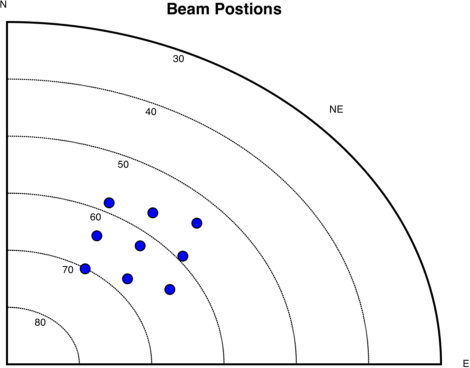
\includegraphics[width=3.5in]{beampositionssts}
%	\caption{A 3x3 grid of desired measurement positions in a
%         hypothetical geodetic latitude/longitude space. }
%	\label{fig:bp1}
%\end{figure}

%\begin{figure}
%	\centering
%	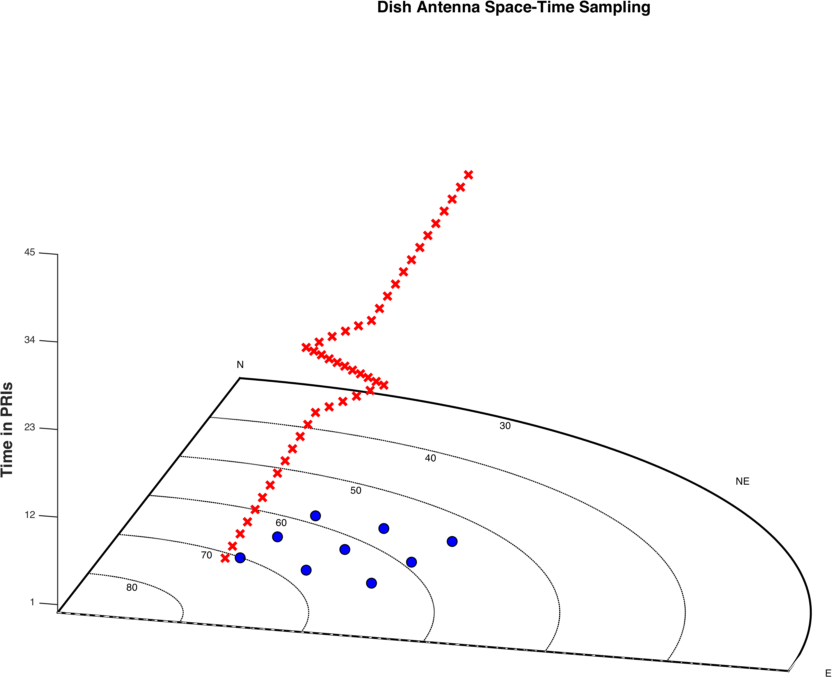
\includegraphics[width=5.5in]{dishsts}
%	\caption{Space-time sampling of the measurement space from Figure~\ref{fig:bp1} using a dish based antenna, where the red x's mark the pulse in beam space and time. Beam positions from Figure \ref{fig:bp1} are shown below in blue at $z=0$.}	
%	\label{fig:dbsts}
%\end{figure}

%\begin{figure}
%	\centering
%	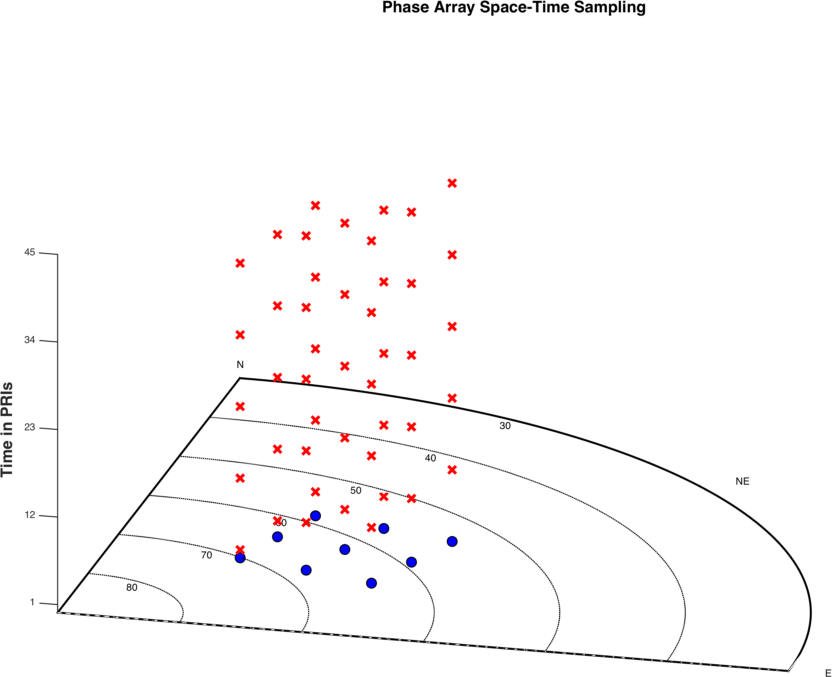
\includegraphics[width=5.5in]{phasedarraysts}
%	\caption{Space-time sampling of the measurement space from Figure~\ref{fig:bp1} using a phased array based antenna, where the red x's mark the pulse in beam space and time. Beam positions from Figure \ref{fig:bp1} are shown below in blue at $z=0$.}	
%	\label{fig:phbsts}
%\end{figure}

The rapid steering ability of ESA systems relative to space-time sampling yields a new flexibility, in post processing, to statistically combine information from different beams using knowledge of the plasma velocity field, where this information is obtained either from external sources or from the Doppler shift of the ionospheric echoes themselves. This can help to relax the assumption of stationarity for plasmas that are evolving or changing their shape on time scales longer than the integration time. If the plasma moves into a different beam, returns from the same plasma can be integrated together with proper bookkeeping. This is contrary to the situation with dish antennas where returns from multiple plasma populations with different parameter sets are unavoidably averaged together.

In order to take advantage of new ESA flexibilities, this work puts forth the idea of the space-time ambiguity function. This concept extends the range ambiguity to all three spatial dimensions along with time. The goal of this paper is to develop a new formalism for treating space-time ambiguity for electronically steerable ISRs, and in particular ISRs that are capable of sampling a given volume on a pulse-by-pulse basis.   This paradigm can also be applied to other types of ISR system designs as well, but much of the utility of using this new formalism is more straightforwardly realized with ESA based systems.  An outline of the paper's development is as follows.  After developing the ambiguity formalism, we will develop specific cases of the impact of the three-dimensional ambiguity on moving plasma using conditions characteristic of polar cap patches. A simulation of a polar cap patch using a full ISR simulator, which creates ISR data at the I/Q level, will be shown. Lastly we will briefly discuss strategies that could improve measurements from electronically steerable ISR systems.

%%%%%%%%%%%%%% Ambiguity Derivation%%%%%%%%%%%%%%%%%%%%%%%%%%%%%%%

\section{Space-Time Ambiguity}

The space-time ambiguity can be thought of as a kernel to a combined volume and time integration operator. In the derivations that follow, we show that this ambiguity can be represented as a kernel operator in a Fredholm integral equation:

\begin{equation}
\label{eqn:friedholm}
\rho(\tau_s ,\mathbf{r}_{s},t_s) = \int L(\tau_s, \mathbf{r}_{s},t_s,\tau,\mathbf{r},t) R(\tau,\mathbf{r},t) dVd t d\tau
\end{equation}

\noindent where, for ISR, $L(\tau_s, \mathbf{r}_{s},t_s,\tau,\mathbf{r},t) $ is a blurring kernel over time and space, and $R(\tau,\mathbf{r},t) $ indicates the plasma medium's autocorrelation function at the lag $\tau$, time $t$, and position $\mathbf{r}$.

By using this formulation, many parallels between ISR and classic camera blurring problems can be made. In cameras, blurring can take place when an object moves over a space covered by one pixel while the shutter is open and the CCD is collecting photons. A diagram of this can be seen in Figure \ref{fig:ccd}. The same holds for the ISR measurement problem, except that the pixels are no longer square or continuous in Cartesian space and instead are determined by the beam shape and pulse pattern. This is shown in the diagrams in Figure \ref{fig:radarblur}.


%\begin{figure}[h!]
%\centering
%	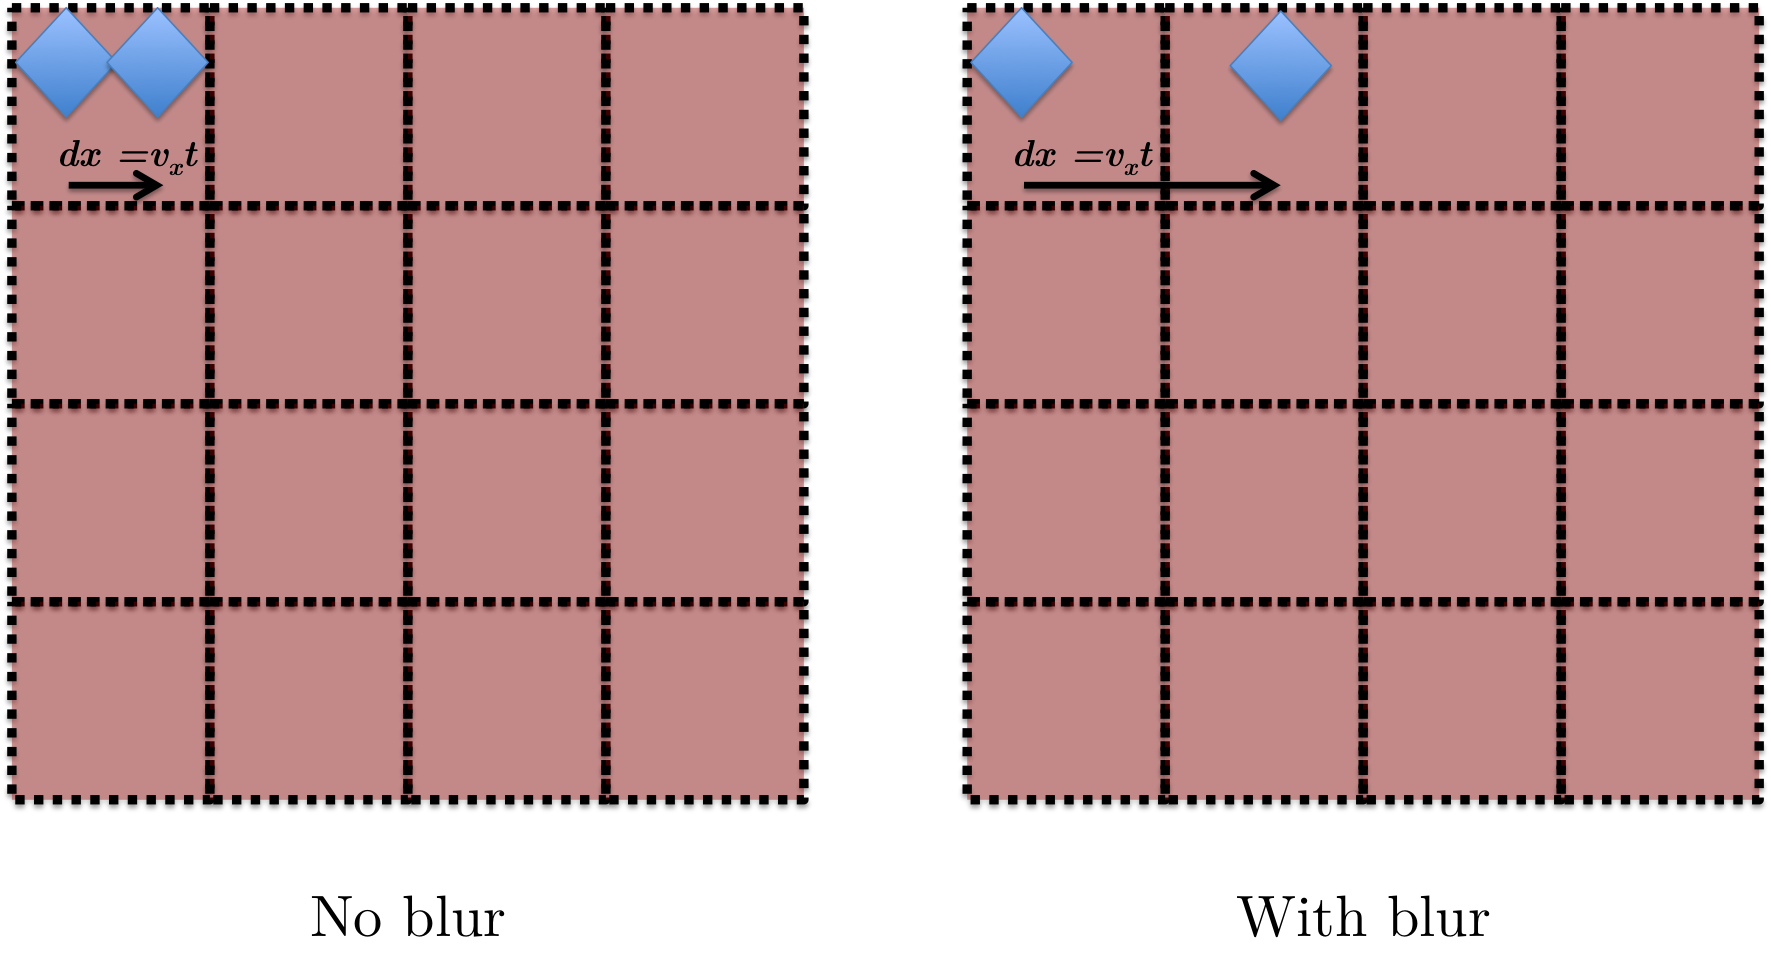
\includegraphics[height=3in]{ccddiagramall}
%	\caption{CCD resolution cell diagram, showing cases where an object will be properly resolved and be blurred.}
%	\label{fig:ccd}
%\end{figure}

%\begin{figure}[h!]
%\centering
%	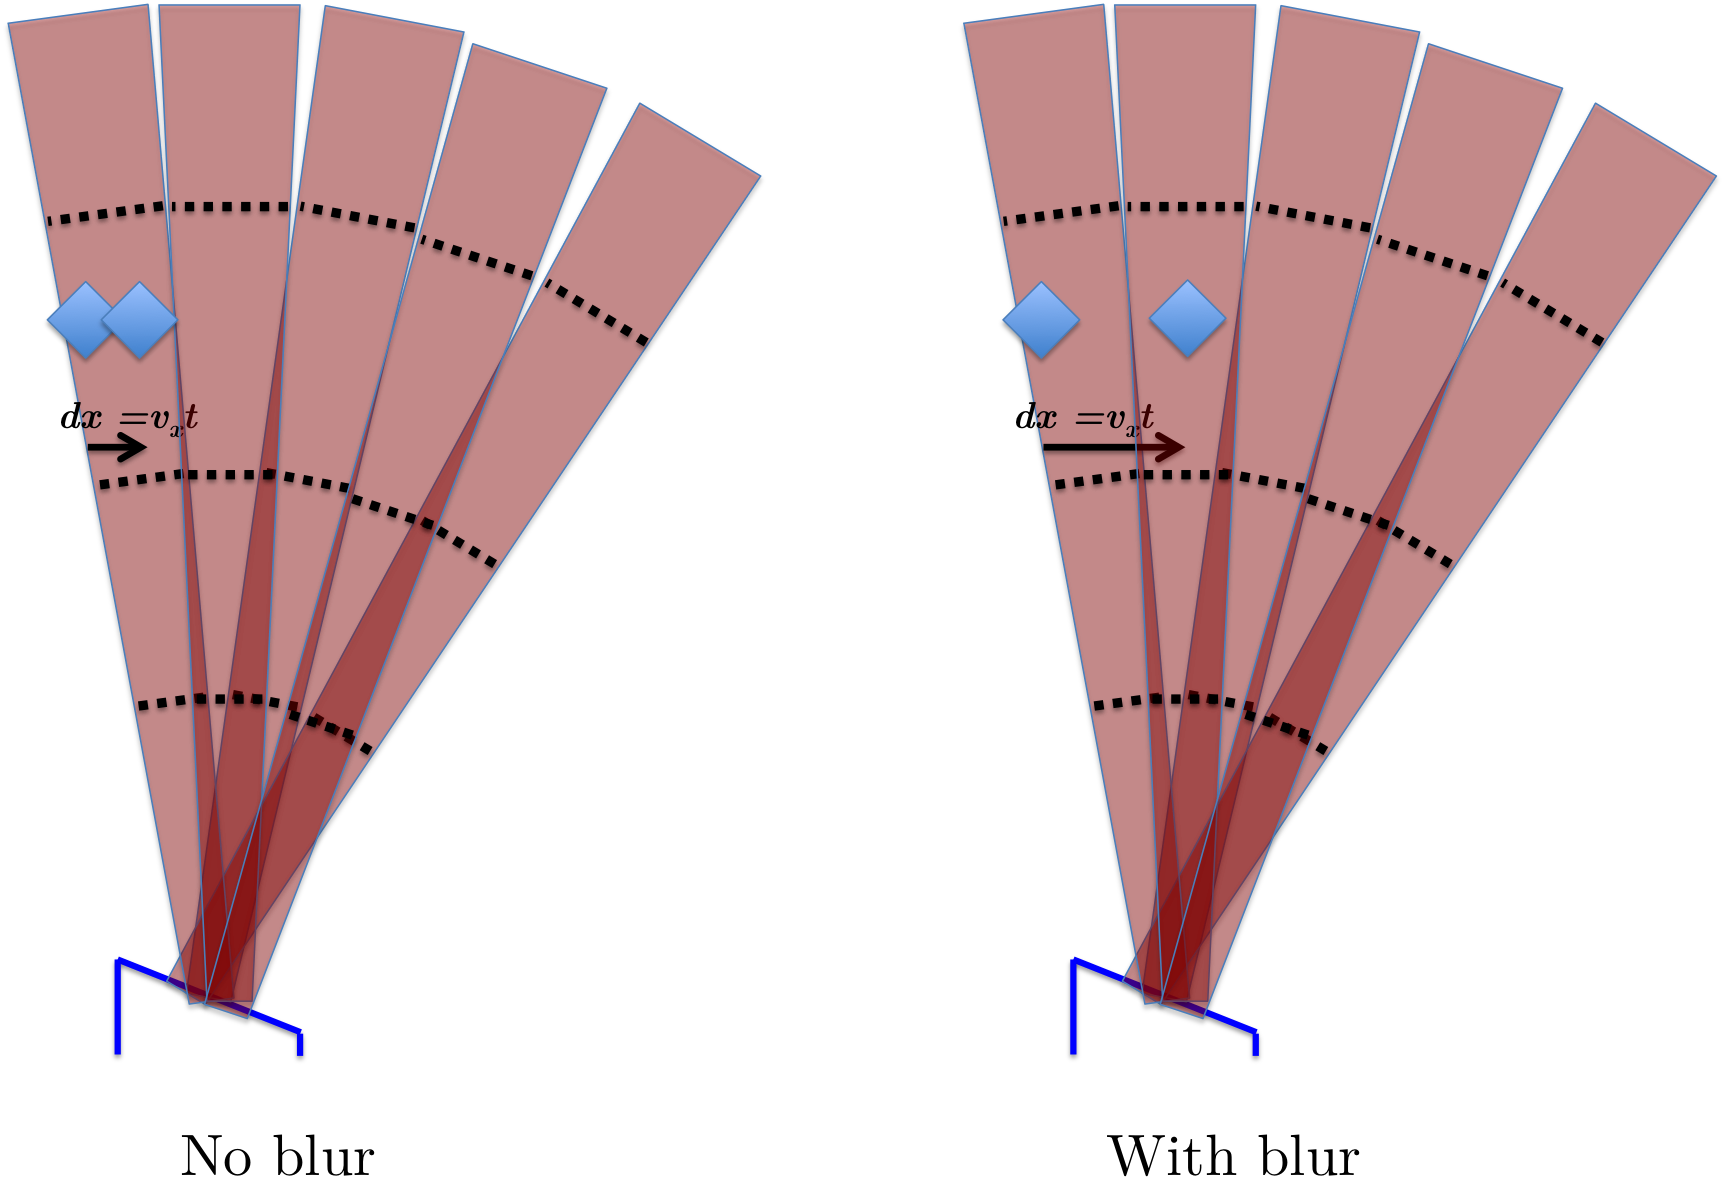
\includegraphics[height=3in]{radardiagramall}
%	\caption{ISR resolution cell diagram, showing cases where an object will be properly resolved and be blurred.}
%	\label{fig:radarblur}
%\end{figure}

\subsection{Coordinate System Definitions}

Before we derive the full space-time ambiguity function, $L(\tau_s,\mathbf{r}_s,t_s,\tau,\mathbf{r},t)$, we will start with defining our coordinate system.  Our three dimensional coordinate system is defined as $\mathbf{r}=[x,y,z]^T$. For this coordinate system, $\mathbf{r}=[0,0,0]^T$ at the location of the radar and thus $r=|\mathbf{r}|$, also known as the range variable. This allows for the use of polar coordinates $\mathbf{r} =  [r,\theta_,\phi]^T$ where $\theta$ and $\phi$ are, respectively, the observer's elevation and azimuth angles.

The radar samples this space at a set of discrete points which will be referred to as $\mathbf{r}_s = [x_s,y_s,z_s]^T$ along with the discretized range expression $r_s=|\mathbf{r}_s|$. The sampled space consists of a number of points, composed of range gates within a beam multiplied by the number of beams. These points can also be referred in polar coordinates $\mathbf{r}_s = [r_s,\theta_s,\phi_s]^T$, where $\theta_s$  and $\phi_s$ are, respectively, the observationally sampled elevation and azimuth angles.

For notation purposes, we use two different sets of time commonly known in the hard-target radar literature as fast-time, $n$ and slow-time, $t$ \cite{richards:fundamentalsigproc}. Fast-time is used to describe processes with correlation time less than one PRI. Slow-time will be used for processes that decorrelate in time on the order of, or longer than, the system's PRI. In order to form estimates of ACFs with desired statistical properties, it is assumed that the plasma parameters parameters will change on the order of many tens to hundreds of PRIs in their stationary reference frame (i.e. remain wide sense stationary for this time). Generally, for incoherent scatter applications in the E-region of the ionosphere ($\approx$100 km altitude) and above, the decorrelation time is less than a PRI for systems with a center frequency in the UHF band, and thus ACFs must be formed over fast-time.

The terms $n$ and $t$ represent continuous variables, while $n_s$ and $t_s$ will be the fast time and slow time parameters sampled by the radar. The sampling rate of $n_s$ is set by the rate at which the system's A/D converters are run. The sampling of $t_s$ can, at the highest rate, be the PRI. At its lowest rate, it can be sampled once in a non-coherent processing interval (NCPI), or equivalently in a period of time it takes the radar to average the desired number of pulses for each beam. 

\subsection{Derivation}

The physical scattering mechanism underlying ISR produces measurable radar scatter from electron density fluctuations in the ionosphere, $n_e(\mathbf{r},n)$, at a specific wavenumber $\mathbf{k}$. These fluctuations scatter radio waves which can be observed by the receiver system of the radar \cite{dougherty:farley1960}. The emitted radar signal at the transmitter has a pulse shape $s(n)$ modulated at a central frequency creating a scattering wave number $\mathbf{k}$. Using the Born approximation, the signal received at time $n$, $x(n)$, can be represented as the following

\begin{equation}
\label{eq:xt}
x(n) = h(n) \ast \int \exp\left[-j\mathbf{k} \cdot \mathbf{r}\right]  s\left(n-\frac{2r}{c}\right) n_e(\mathbf{r},n) d\mathbf{r},
\end{equation}

\noindent where $h(n)$ is the receiver filter and the $\ast$ represents the convolution operator. In modern ISR systems, this signal $x(n)$ is then sampled at discrete points in fast-time which will be referred to as $n_s$. The convolution and sampling operation can be brought in the integral as the following,

\begin{equation}
\label{ex:xtaug}
x(n_s) = \int \exp\left[-j\mathbf{k} \cdot \mathbf{r}\right]  s\left(n-\frac{2r}{c}\right) n_e(\mathbf{r},n)h(n_s-n) d\mathbf{r}dn
\end{equation}


Once the signal has been received and sampled, the autocorrelation function is then estimated from the sampled signal $x(n_s)$. The full expression of the underlying autocorrelation of this signal is the following, 

\begin{multline}
\label{ex:acf0}
\langle x(n_s)x^*(n_s')\rangle =  \int \exp\left[-j \mathbf{k}\cdot \left(\mathbf{r}'-\mathbf{r} \right)\right]s\left(n-\frac{2r}{c}\right)s^*\left(n'-\frac{2r'}{c}\right) \\ h(n_s-n)h(n_s'-n')\langle n_e(\mathbf{r},n)n^*_e(\mathbf{r}',n')\rangle d\mathbf{r} d\mathbf{r}'dn dn',
\end{multline}

\noindent where $r'$ is the magnitude of the vector $\mathbf{r}'$. By assuming stationarity of second order signal statistics along fast time, we can then substitute the lag variables $\tau\equiv n'-n$, and $\tau_s\equiv n_s'-n_s$. With these substitutions, Equation \ref{ex:acf0} becomes


\begin{multline}
\label{ex:acf1}
\langle x(n_s)x^*(n_s+\tau_s)\rangle =\int \exp\left[-j \mathbf{k}\cdot \left(\mathbf{r}'-\mathbf{r} \right)\right]s\left(n-\frac{2r}{c}\right)s^*\left(n+\tau-\frac{2r'}{c}\right) \\ h(n_s-n)h(n_s+\tau_s-n-\tau) \langle n_e(\mathbf{r},n)n^*_e(\mathbf{r}',n+\tau)\rangle d\mathbf{r} d\mathbf{r}' dnd\tau
\end{multline}

\noindent We can make a simplifying assumption at this point that the space-time autocorrelation function of $n_e(\mathbf{r},t)$, $\langle n_e(\mathbf{r},n)n_e(\mathbf{r}',n+\tau)\rangle$, will go to zero as the magnitude of $\mathbf{y} \equiv \mathbf{r}'-\mathbf{r}$ increases beyond the debye length \cite{farley1969}. Thus, the rate which the spatial autocorrelation goes to zero will be such that $\tau\gg \frac{2||\mathbf{y}||}{c}$, allowing us to set $r= r'$ inside the arguments of $s$ and $h$. This allows Equation \ref{ex:acf1} to be rewritten as 
 
 \begin{multline}
 \label{ex:acf2}
 \langle x(n_s)x^*(n_s+\tau)\rangle = \int s\left(n-\frac{2r}{c}\right)s^*\left(n+\tau -\frac{2r}{c}\right) h(n_s-n)h^*(n_s+\tau_s-n-\tau) \\\left[\int \exp\left[-2j \mathbf{k}\cdot \mathbf{y}\right] \langle n_e(\mathbf{r},n)n^*_e(\mathbf{y}+\mathbf{r},n+\tau)\rangle d\mathbf{y} \right]drdn d\tau.
 \end{multline}

The inner integral is a spatial Fourier transform evaluated at the wave number of the radar $\mathbf{k}$. By again asserting stationarity along fast time, we can represent the true ACF as the following,
 \begin{equation}
 \label{eq:spft}
R(\tau,\mathbf{r})= \langle |n_e(\mathbf{k},r,\tau)|^2\rangle \equiv  \int \exp\left[-2j \mathbf{k}\cdot \mathbf{y} \right] \langle n_e(\mathbf{r},b)n^*_e(\mathbf{y}+\mathbf{r},n+\tau)\rangle d\mathbf{y}.
 \end{equation}
 
 \noindent Now Equation \ref{ex:acf2} becomes
 
 \begin{equation}
 \langle x(n_s)x^*(n_s+\tau_s)\rangle = \int \langle |n_e(\tau,\mathbf{k},\mathbf{r})|^2\rangle\left[\int s(n-\frac{2r}{c})s^*(n+\tau -\frac{2r}{c})h(n_s-n)h^*(n_s+\tau_s-n-\tau) dn \right]d\tau dr.
 \end{equation}

 If $n_s$ is replaced with $2r_s/c$ we can introduce the range ambiguity function $W(\tau_s,r_s,\tau,r)$ by doing the following substitution,
 \begin{equation}
 \label{eqn:rngamb}
 W(\tau_s,r_s,\tau,r)= \int s(n-\frac{2r}{c})s^*(n+\tau -\frac{2r}{c})h(2r_s/c-n)h^*(2r_s/c+\tau_s-n-\tau) dn.
 \end{equation}
 
Assuming, for the moment, that $R(\tau,\mathbf{r})$ only varies across the range dimension $r$, we can now represent this in the form of a Fredholm integral equation
 
 \begin{equation}
 \label{eqn:fredfirst}
 \langle x(2r_s/c)x^*(2r_s/c+\tau_s)\rangle = \int W(\tau_s,r_s,\tau,r)R(\tau,r) drd\tau.
 \end{equation}
 
\noindent The range ambiguity function, $W(\tau_s,r_s,\tau,r)$, can be thought of as a smoothing operator along the range and lag dimensions of $R(\tau,r)$. This result is also derived in \cite{nikoukar2008}, \cite{Woodman:1991is} and \cite{hysell2008}

 
The spatial ambiguity across azimuth and elevation angles is determined by the antenna beam pattern. In phased array antennas, this beam pattern is ideally the array factor multiplied by the element pattern \cite{Balanis:2005:ATA:1208379}. The array factor is determined by a number of things including the element spacing and the wave number of the radar, $k$. For example, by making idealized assumptions with no mutual coupling and that the array elements are simple cross dipole elements, AMISR systems will have the following antenna pattern for pointing angle ($\theta_s,\phi_s$): 

 \begin{equation}
 \label{eqn:amisrpat}
F(\theta_s,\phi_s,\theta,\phi) = \frac{1}{2}(1+\cos(\theta)^2)\left[ \frac{1}{MN} \left(1+\exp\left[j(\psi_y/2 + \psi_x)\right]\right)\frac{\sin((M/2) \psi_x)}{\sin(\psi_x)} \frac{\sin((N/2) \psi_x)}{\sin(\psi_x/2)}\right]^2,
 \end{equation}
 
 \noindent where $\psi_x = -k d_x(\sin\theta\cos\phi-\sin\theta_s\cos\phi_s)$, $\psi_y = -k d_y(\sin\theta\sin\phi-\sin\theta_s\sin\phi_s)$ and $M$ is the number of elements in the $x$ direction of the array, and $N$ is the number of elements in the $y$ direction(see Appendix: \ref{App:AMISRarr} for derivation).


The spatial ambiguity is a separable function made up of the components of $W(\tau_s,\tau,r_s,r)$ and $F(\theta_s,\phi_s,\theta,\phi)$. These two functions can be combined by multiplying the two, creating the spatial ambiguity function  $K(\tau_s,\mathbf{r}_s,\tau,\mathbf{r})$. This yields an expression for a single statistical realization of the ACF of the incoherent scatter random process, which will be referred to as $\rho(\tau_s,\mathbf{r}_s)$:


 \begin{align}
  \label{eqn:volume}
\rho(\tau_s,\mathbf{r}_s) &= \int F(\theta_s,\phi_s,\theta,\phi)W(\tau_s,r_s,\tau,r) R(\tau,\mathbf{r}) dV d\tau ,\\
	&= \int K(\tau_s,\mathbf{r}_s,\tau,\mathbf{r}) R(\tau,\mathbf{r})  dVd\tau.
\end{align}

A rendering of an example of this full spatial ambiguity function for an uncoded long pulse, with antenna pattern from Equation \ref{eqn:amisrpat} for four beams, can be seen in Figure \ref{fig:amb4}.

%\begin{figure}
%	\centering
%	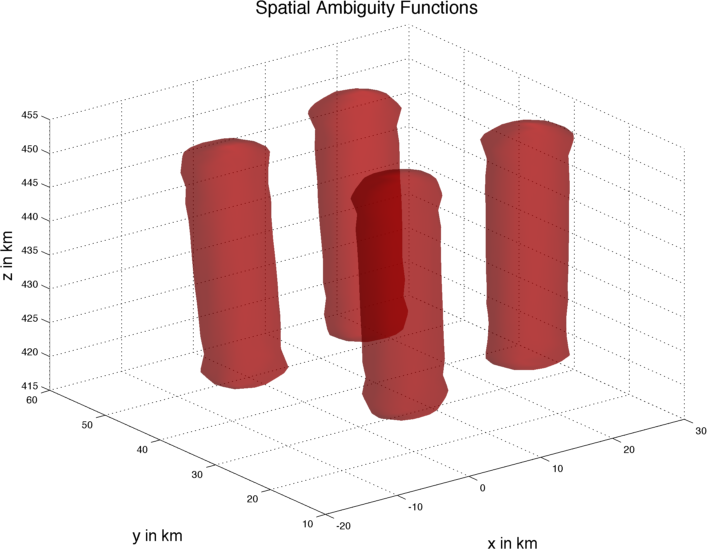
\includegraphics[width=5.5in]{spaceamb}
%	\caption{Full spatial ambiguity function in Cartesian space for case with 4 beams with trailing edge of a 240$\mu$s pulse at 400km range. The surface represents the half power point of the ambiguity function.}	
%	\label{fig:amb4}
%\end{figure}

As mentioned above, this one pulse ACF estimate represents a single sample of a random process. In order to create a usable estimate, multiple samples of this ACF need to be averaged together to reduce the variance to sufficient levels in order to fit the estimate to a theoretical ACF that is a direct function of plasma parameter values. To show the impact of this averaging in creating the estimate of the ACF, we will add slow-time dependence to the expression for the medium ACF, which now becomes $R(\tau,\mathbf{r},t)$, and will also add another separable function $G(t_s,t)$ to the kernel. This function $G(t_s,t)$ can be thought of as a sampling and blurring kernel for the ACF if the plasma parameters change within an NCPI. Since the amount of time that the radar pulse is illuminating the plasma in a point of space is very short compared to the PRI, $G(t_s,t)$ can take the form of a summation of Dirac delta functions 

\begin{equation}
\label{eqn:Gexp}
G(t_s,t) = \displaystyle \sum_{j=0}^{J-1}\alpha_j \delta(t-t_s-jT_{REV}),
\end{equation}

\noindent where $J$ counts the number of pulses used over a NCPI, $T_{REV}$ is the amount of time it takes the radar to revisit the specific beam and $\alpha_j$ represent the weights that the radar assigns to the pulses. For systems using pulse-to-pulse steering, one strategy revisits each beam sequentially, in this case making $T_{REV}=N_{beam}T_{PRI}$, where $N_{beam}$ is the number of beams and $T_{PRI}$ is the PRI time period. For the case where weights are set to $1/J$, this operation simply averages the pulses. With Equation \ref{eqn:Gexp} incorporated into the overall ambiguity we obtain the full integral equation,

\begin{equation}
\label{eqn:sptamb}
	\rho(\tau_s,\mathbf{r}_s,t_s) =\int L(\tau_s,\mathbf{r}_s,t_s,\tau,\mathbf{r},t)R(\tau,\mathbf{r},t)dVdtd\tau.
\end{equation}

\noindent The final kernel, $L(\tau_s,\mathbf{r}_s,t_s,\tau,\mathbf{r},t) = G(t_s,t)K(\tau_s,\mathbf{r}_s,\tau,\mathbf{r})$, encompasses the full space-time ambiguity.

\subsection{Ambiguity after Frame Transformation}

We will now focus on the impact of the motion of plasma as it is going through the field of view of the radar. We will assume that the radar is integrating over a length of time $T$ beginning at $t_s$. The kernel $L$ will be represented as a separable function $K$ and $G$ as in Equation \ref{eqn:sptamb}. In this case, $G$ will be a summation of Dirac delta functions with weights of $1/J$. This will change Equation \ref{eqn:sptamb} to the following:

\begin{equation}
\label{eqn:L2}
\rho(\tau_s,\mathbf{r}_s,t_s) = \int K(\tau_s,\mathbf{r}_s,\tau,\mathbf{r}) \left[(1/J)\int_{t_s}^{t_s+T} \displaystyle \sum_{j=0}^{J-1} \delta(t-t_s-jT_{REV})R(\tau,\mathbf{r},t) dt\right] dVd\tau.
\end{equation}

Of specific interest in this study are instances in the high latitude ionosphere where embedded plasma structures are moving due to electric field drivers applied by the magnetosphere. In this case, it will be assumed that the plasma is a rigid object and will not deform with respect to $\mathbf{r}$ over time period $[t_0,t_0+T]$ where $T=JT_{REV}$ is the time for one NCPI. Also, it will be assumed that the plasma parcel moves with a constant velocity $\mathbf{v}$. Thus $R(\tau,\mathbf{r},t)\Rightarrow R(\tau,\mathbf{r}+\mathbf{v}t)$. The assumption of rigidity can in some cases be valid over the time period of the NCPI, on the order of a few minutes, while the plasma moves through the field of view of the radar. For example, in the high latitude ionosphere, large scale features in structures such as patches decay on the order of hours \cite{Tsunoda:1988ul}. This assumption is useful because it allows our framework to analyze impacts of these plasma variations on the parameter resolution of ISR systems. With these assumptions, Equation \ref{eqn:L2} becomes,

\begin{equation}
\label{eqn:L3}
\rho(\tau_s,\mathbf{r}_s,t_s) =(1/J) \int \int_{t_s}^{t_s+T} \displaystyle \sum_{j=0}^{J-1}\delta(t-t_s-jT_{REV}) K(\tau_s,\mathbf{r}_s,\tau,\mathbf{r})R(\tau,\mathbf{r}+\mathbf{v}t)dtdVd\tau\end{equation}

A change of variables to $\mathbf{r}' = \mathbf{r}+\mathbf{v}t$ acts as a Galilean transform and applies a warping to the kernel, changing the frame of reference. Since $R(\tau,\mathbf{r}')$ is no longer dependent on $t$, Equation \ref{eqn:L3} can be integrated in time and becomes:

\begin{equation}
\label{eqn:L5}
\rho(\tau_s,\mathbf{r}_s,t_s)= (1/J)\int \left[ \;\;  \displaystyle \sum_{j=0}^{J-1} K(\tau_s,\mathbf{r}_s,\tau,\mathbf{r}'-\mathbf{v}(t_s+jT_{REV})) \;\; \right]R(\tau,\mathbf{r}')dVd\tau.
\end{equation}

The problem can now be simplified further back to a Fredholm integral equation by simply replacing the terms in the square brackets as a new kernel $A(\tau_s,\mathbf{r}_s,t_s,\tau,\mathbf{r}')$:

\begin{equation}
\label{eqn:L6}
\rho(\tau_s,\mathbf{r}_s,t_s)= \int A(\tau_s,\mathbf{r}_s,t_s,\tau,\mathbf{r}') R(\tau,\mathbf{r}')dVd\tau.
\end{equation}

\noindent The impact of the plasma velocity on the ambiguity function can be seen in Figure \ref{fig:ambtime}. This is the same ambiguity as seen in Figure \ref{fig:amb4} but with a velocity of 500 m/s in the $y$ direction over a period of 2 minutes. This velocity creates a larger ambiguity function in the frame of reference of the moving plasma.

%\begin{figure}[!t]
%	\centering
%	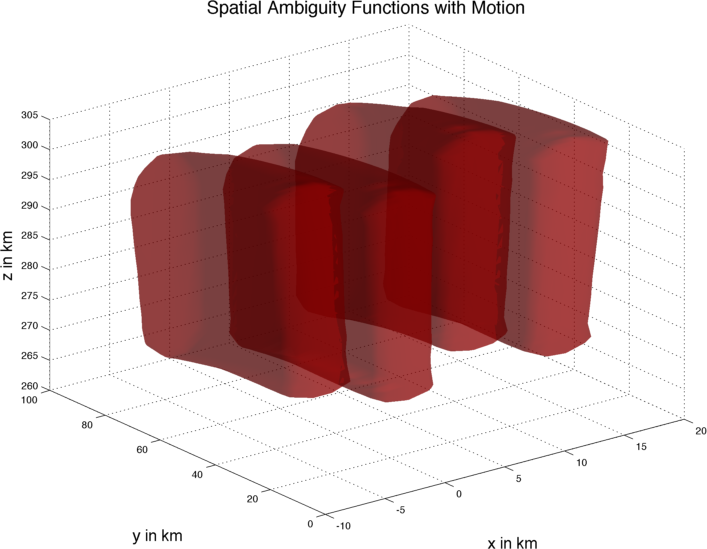
\includegraphics[width=5.5in]{spaceambmoving}
%	\caption{Same spatial ambiguity as in Figure \ref{fig:amb4} but now with 500 m/s velocity in $y$ direction in plasma frame of reference. The surface represents the half power point of the ambiguity function.}
%	\label{fig:ambtime}
%\end{figure}

The operator $A$ can be determined through knowledge of the radar system's beam pattern along with the experiment's pulse pattern, integration time and inherent velocity of the plasma. This velocity $\mathbf{v}$ could be separately estimated by taking measurements of the Doppler shift by using a methodology like that seen in \cite{butler:imagingfregiondrifts}. With this strategy, the operator is now acting purely as a spatial blurring function instead of a full space-time function. We note that reducing dimensionality of the problem can make it easier to solve the inverse problem in practice.
